\documentclass[tikz, border=10pt]{standalone}

% Schriftart-Einstellungen gemäß Vorgabe
\usepackage{tgheros}
\renewcommand{\familydefault}{\sfdefault}

% TikZ-Bibliotheken
\usetikzlibrary{positioning, shapes, calc}

% Zentrale Stil-Definitionen
\tikzset{
    punkt/.style={
        circle,
        draw=black,          % Klare schwarze Kontur
        fill=white,          % Neutrale weiße Füllung
        minimum size=3.5mm,  % Definierte Größe für perfekte Kreise
        line width=0.7pt     % Professionelle Linienstärke
    }
}

\begin{document}
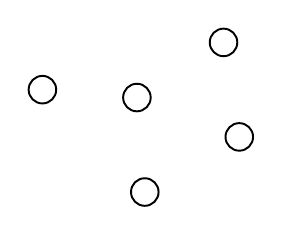
\begin{tikzpicture}

    % Platzierung der 5 Punkte basierend auf der visuellen Analyse der Handskizze:
    % Die Anordnung ist bewusst unregelmäßig gehalten, um den Charakter 
    % des Originals beizubehalten, während die Formen geometrisch perfekt sind.

    % Zentraler/Oberer Punkt
    \node[punkt] (P1) at (0,0) {}; 
    
    % Punkt oben rechts
    \node[punkt] (P2) at (1.1, 0.7) {};
    
    % Punkt unten rechts
    \node[punkt] (P3) at (1.3, -0.5) {};
    
    % Punkt unten mittig
    \node[punkt] (P4) at (0.1, -1.2) {};
    
    % Punkt links
    \node[punkt] (P5) at (-1.2, 0.1) {};

\end{tikzpicture}
\end{document}